\documentclass[11pt,a4paper]{article}
\usepackage[utf8]{inputenc}
\usepackage[T1]{fontenc}
\usepackage{lmodern}
\usepackage{graphicx}
\usepackage{amsmath}
\usepackage{booktabs}
\usepackage{hyperref}
\usepackage{caption}
\usepackage{subcaption}
\usepackage{geometry}
\geometry{margin=1in}

\title{Comprehensive Regression Analysis of Key U.S. Economic Indicators\\
\large Based on FRED Data (2010–2025)}
\author{David Nguyen \\ University of North Carolina at Chapel Hill}
\date{April 8, 2025}

\begin{document}

\maketitle

\begin{abstract}
  This report presents a detailed statistical analysis of fourteen major U.S. economic time series obtained from the Federal Reserve Economic Data (FRED) API. We apply linear, polynomial (where relevant), logarithmic, and percent‐change regressions to each series, evaluate model fit via \(R^2\), and illustrate results with plots. The aim is to identify robust trends, assess model suitability, and provide actionable economic insights.
\end{abstract}

\tableofcontents
\clearpage

\section{Introduction}
Economic policymakers and financial analysts rely on accurate trend estimation to guide decisions. Here, we examine fourteen series covering banking, production, prices, rates, and markets, spanning January 2010 through April 2025. We compare regression forms to determine which best captures long‐term behavior.

\section{Data \& Methodology}
\subsection{Data Acquisition}
Data were fetched via the FRED API and stored in MongoDB. Each time series was converted to a numerical index \(t\) measured as days since its first observation.

\subsection{Regression Models}
For each series \(y(t)\):
\begin{itemize}
  \item \textbf{Linear:} \(y = \beta_1 t + \beta_0\)
  \item \textbf{Polynomial (order 2):} \(y = \alpha_2 t^2 + \alpha_1 t + \alpha_0\) (only for TOTALSL)
  \item \textbf{Logarithmic:} \(y = \gamma_1 \ln(t) + \gamma_0\)
  \item \textbf{Percent‐change:} regress \(\Delta y / y_{t-1}\) versus index
\end{itemize}
Model performance is evaluated via the coefficient of determination \(R^2\).

\subsection{Visualization}
Plots were generated and saved under \texttt{backend/analyses/*.png}. Each subsection below embeds the linear and logarithmic fit figures; TOTALSL also includes the second‐order polynomial fit.

\clearpage
\section{Results by Series}

\subsection{TOTALSL: Total Loans \& Leases at Commercial Banks}
\textbf{Time Period:} January 1, 2010 – February 1, 2025 (182 observations)

\begin{itemize}
  \item \textbf{Linear regression:} \(y = 496.0598\,t + 2{,}404{,}193.2494\), \(R^2 = 0.9912\).
  \item \textbf{Polynomial (order 2):} \(R^2 = 0.9900\). Orders 3–10 yield negative \(R^2\) (overfitting).
  \item \textbf{Percent‐change regression:} \(y = -0.005\,t + 0.4397\), \(R^2 = 0.0189\).
  \item \textbf{Logarithmic regression:} \(y = 1{,}454{,}435.8907\,\ln(t) + 384{,}818.869\), \(R^2 = 0.6106\).
\end{itemize}

\begin{figure}[htbp]
  \centering
  \begin{subfigure}[b]{0.32\textwidth}
    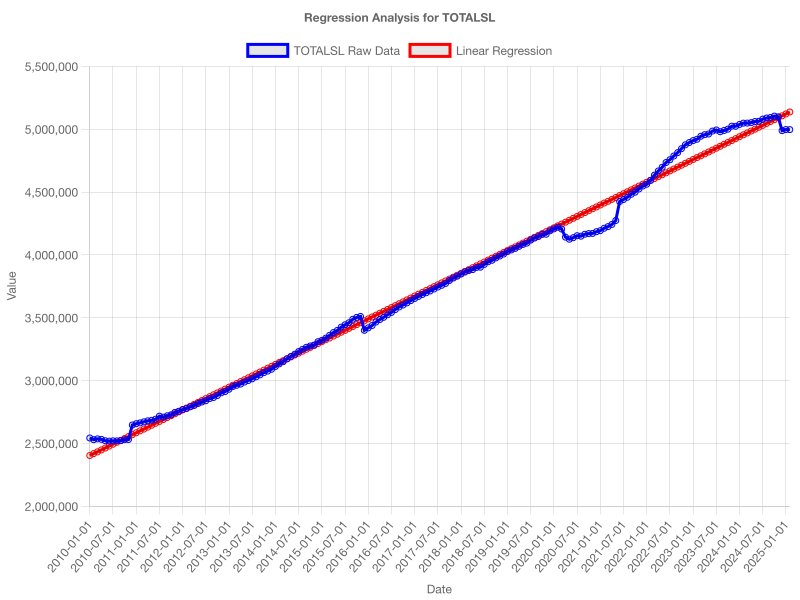
\includegraphics[width=\textwidth]{backend/analyses/TOTALSL_analysis.png}
    \caption{Linear Fit}
  \end{subfigure}
  \hfill
  \begin{subfigure}[b]{0.32\textwidth}
    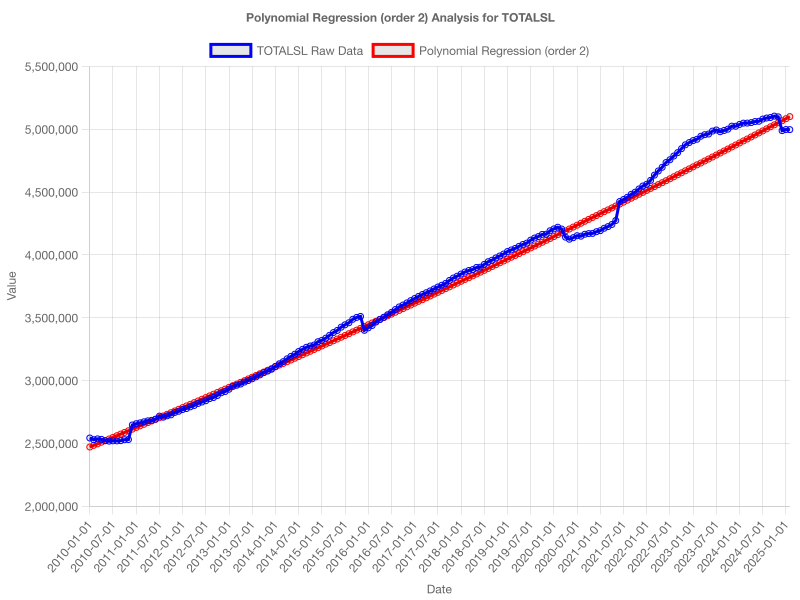
\includegraphics[width=\textwidth]{backend/analyses/TOTALSL_poly_order_2_analysis.png}
    \caption{Polynomial Order 2}
  \end{subfigure}
  \hfill
  \begin{subfigure}[b]{0.32\textwidth}
    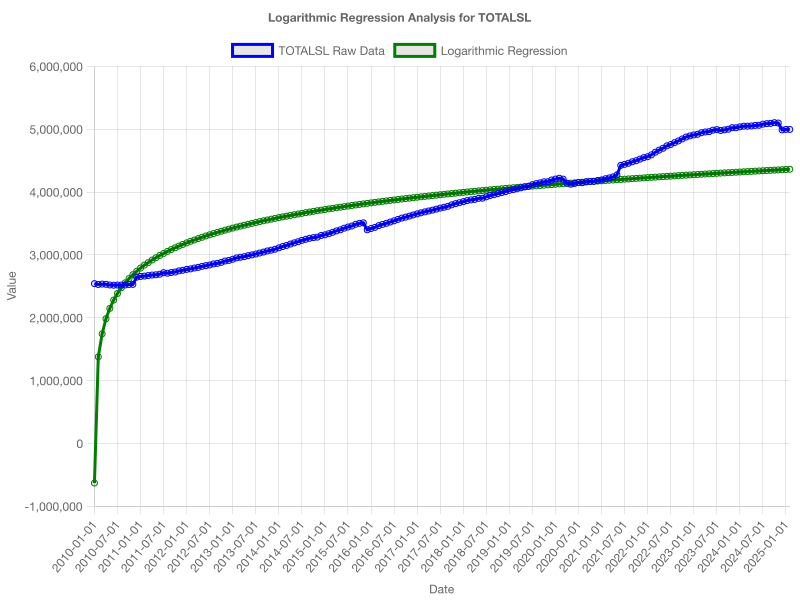
\includegraphics[width=\textwidth]{backend/analyses/TOTALSL_log_analysis.png}
    \caption{Logarithmic Fit}
  \end{subfigure}
  \caption{Regression Analyses for TOTALSL}
\end{figure}

\paragraph{Summary:}
A very strong linear trend explains over 99\% of the variance. The second‐order polynomial adds negligible improvement, while higher orders overfit. Percent‐change and logarithmic models perform poorly relative to linear.

\clearpage
\subsection{TOTALSA: Total Assets of Commercial Banks}
\textbf{Time Period:} January 1, 2010 – March 1, 2025 (183 observations)

\begin{itemize}
  \item \textbf{Linear regression:} \(y = 0.0009\,t + 14.5552\), \(R^2 = 0.0843\).
  \item \textbf{Polynomial regressions (orders 2–10):} negative \(R^2\), indicating misfit.
  \item \textbf{Percent‐change regression:} \(y = 0.0023\,t + 0.2811\), \(R^2 \approx 0.0000\).
  \item \textbf{Logarithmic regression:} \(y = 20.8478\,\ln(t) - 0.5993\), \(R^2 = 0.1646\).
\end{itemize}

\begin{figure}[htbp]
  \centering
  \begin{subfigure}[b]{0.48\textwidth}
    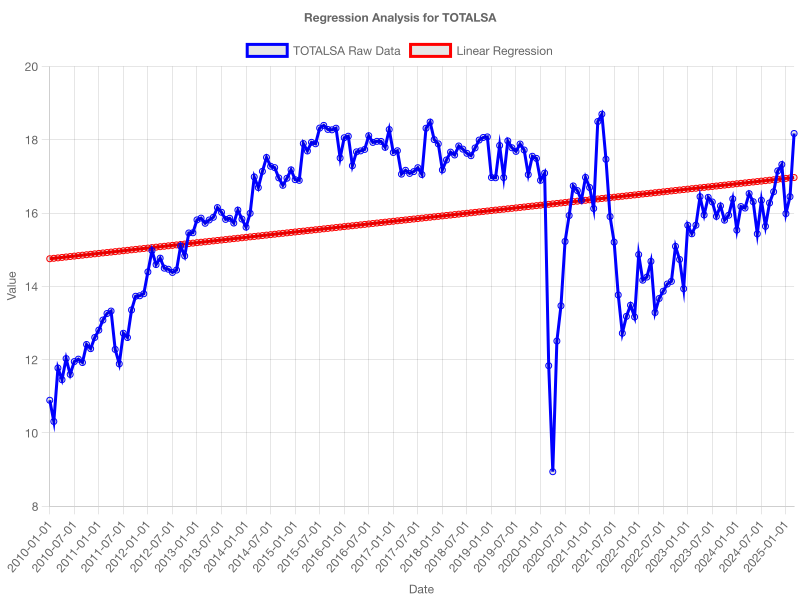
\includegraphics[width=\textwidth]{backend/analyses/TOTALSA_analysis.png}
    \caption{Linear Fit}
  \end{subfigure}
  \hfill
  \begin{subfigure}[b]{0.48\textwidth}
    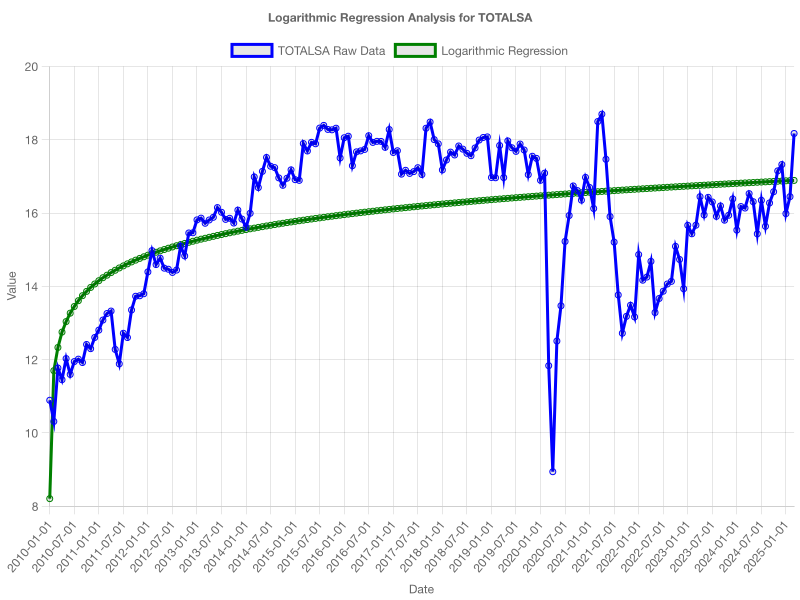
\includegraphics[width=\textwidth]{backend/analyses/TOTALSA_log_analysis.png}
    \caption{Logarithmic Fit}
  \end{subfigure}
  \caption{Regression Analyses for TOTALSA}
\end{figure}

\paragraph{Summary:}
All models explain little variance; further covariates or alternative approaches are needed.

\clearpage
\subsection{MPRIME: Bank Prime Loan Rate}
\textbf{Time Period:} January 1, 2020 – February 1, 2025 (62 observations)

\begin{itemize}
  \item \textbf{Linear regression:} \(y = 0.0037\,t + 2.2573\), \(R^2 = 0.7678\).
  \item \textbf{Polynomial regressions (orders 2–10):} negative \(R^2\).
  \item \textbf{Percent‐change regression:} \(y = 0.0396\,t - 0.3106\), \(R^2 = 0.0198\).
  \item \textbf{Logarithmic regression:} \(y = -1.1371\,\ln(t) + 0.8515\), \(R^2 = 0.2596\).
\end{itemize}

\begin{figure}[htbp]
  \centering
  \begin{subfigure}[b]{0.48\textwidth}
    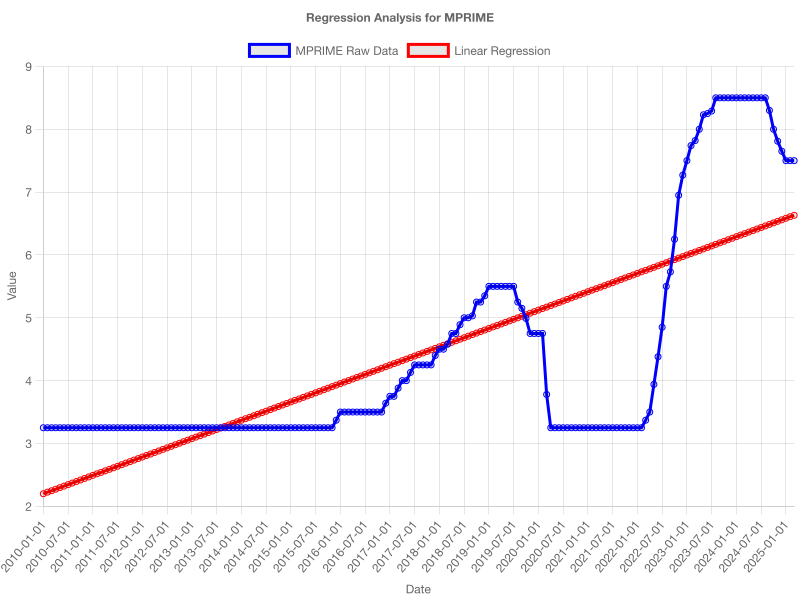
\includegraphics[width=\textwidth]{backend/analyses/MPRIME_analysis.png}
    \caption{Linear Fit}
  \end{subfigure}
  \hfill
  \begin{subfigure}[b]{0.48\textwidth}
    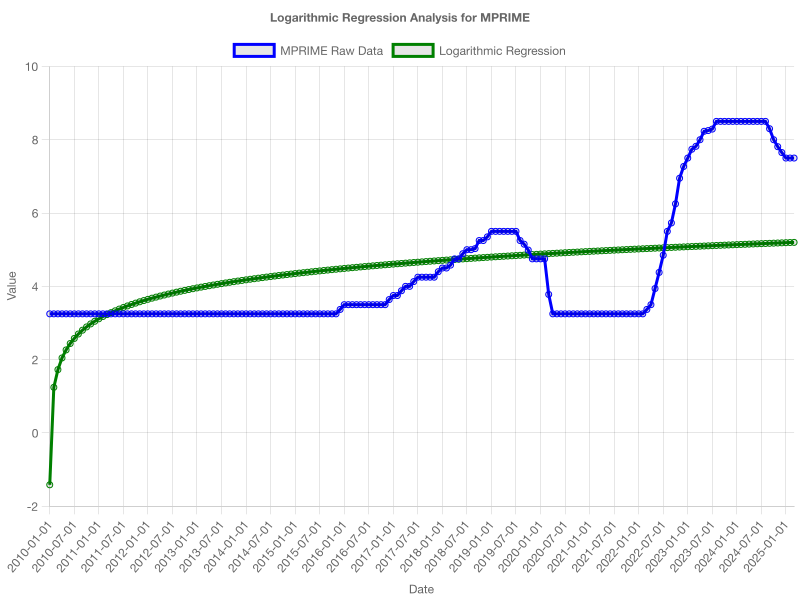
\includegraphics[width=\textwidth]{backend/analyses/MPRIME_log_analysis.png}
    \caption{Logarithmic Fit}
  \end{subfigure}
  \caption{Regression Analyses for MPRIME}
\end{figure}

\paragraph{Summary:}
Linear model is robust; other forms underperform.

\clearpage
\subsection{FEDFUNDS: Effective Federal Funds Rate}
\textbf{Time Period:} January 1, 2020 – February 1, 2025 (62 observations)

\begin{itemize}
  \item \textbf{Linear regression:} \(y = 0.0037\,t - 0.9124\), \(R^2 = 0.7680\).
  \item \textbf{Polynomial regressions:} negative \(R^2\).
  \item \textbf{Percent‐change regression:} \(y = 0.0346\,t + 6.7420\), \(R^2 = 0.0003\).
  \item \textbf{Logarithmic regression:} \(y = -4.1822\,\ln(t) + 0.8384\), \(R^2 = 0.2544\).
\end{itemize}

\begin{figure}[htbp]
  \centering
  \begin{subfigure}[b]{0.48\textwidth}
    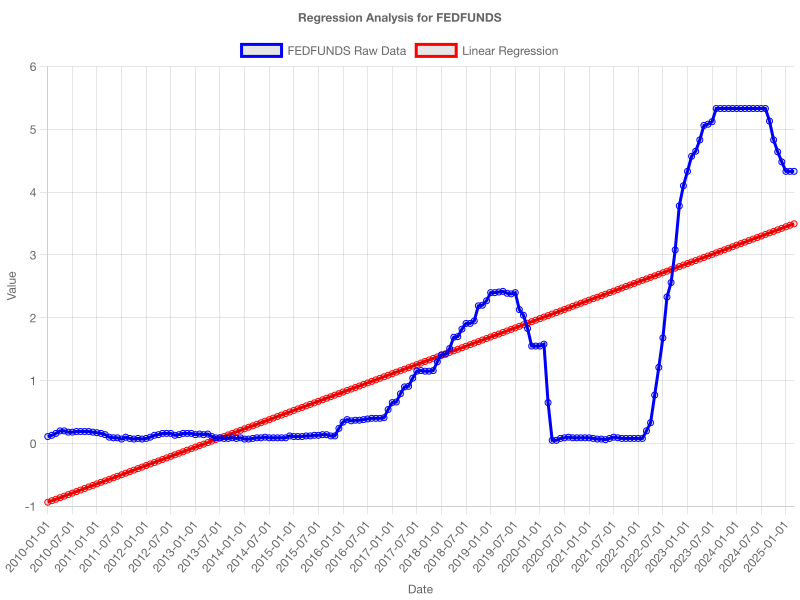
\includegraphics[width=\textwidth]{backend/analyses/FEDFUNDS_analysis.png}
    \caption{Linear Fit}
  \end{subfigure}
  \hfill
  \begin{subfigure}[b]{0.48\textwidth}
    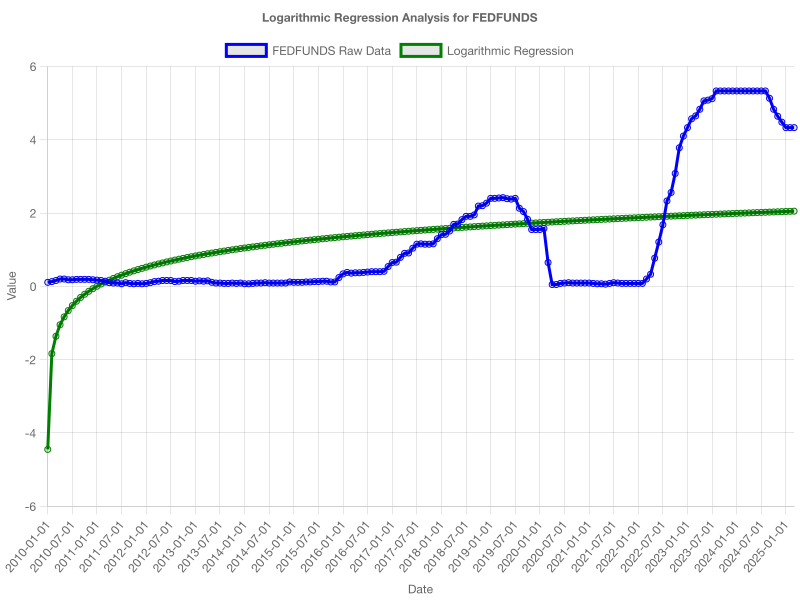
\includegraphics[width=\textwidth]{backend/analyses/FEDFUNDS_log_analysis.png}
    \caption{Logarithmic Fit}
  \end{subfigure}
  \caption{Regression Analyses for FEDFUNDS}
\end{figure}

\paragraph{Summary:}
Linear model captures most of the variance; others fail.

\clearpage
\subsection{INDPRO: Industrial Production Index}
\textbf{Time Period:} January 1, 2010 – February 1, 2025 (182 observations)

\begin{itemize}
  \item \textbf{Linear regression:} \(y = 0.0014\,t + 95.7155\), \(R^2 = 0.3463\).
  \item \textbf{Polynomial regressions:} negative \(R^2\).
  \item \textbf{Percent‐change regression:} \(y = -0.0011\,t + 0.1942\), \(R^2 = 0.0018\).
  \item \textbf{Logarithmic regression:} \(y = 81.6334\,\ln(t) + 2.3627\), \(R^2 = 0.4797\).
\end{itemize}

\begin{figure}[htbp]
  \centering
  \begin{subfigure}[b]{0.48\textwidth}
    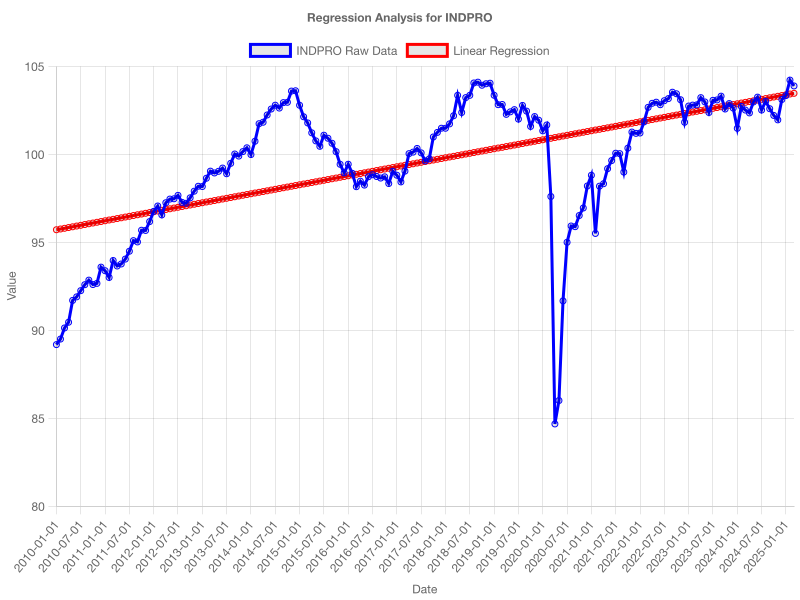
\includegraphics[width=\textwidth]{backend/analyses/INDPRO_analysis.png}
    \caption{Linear Fit}
  \end{subfigure}
  \hfill
  \begin{subfigure}[b]{0.48\textwidth}
    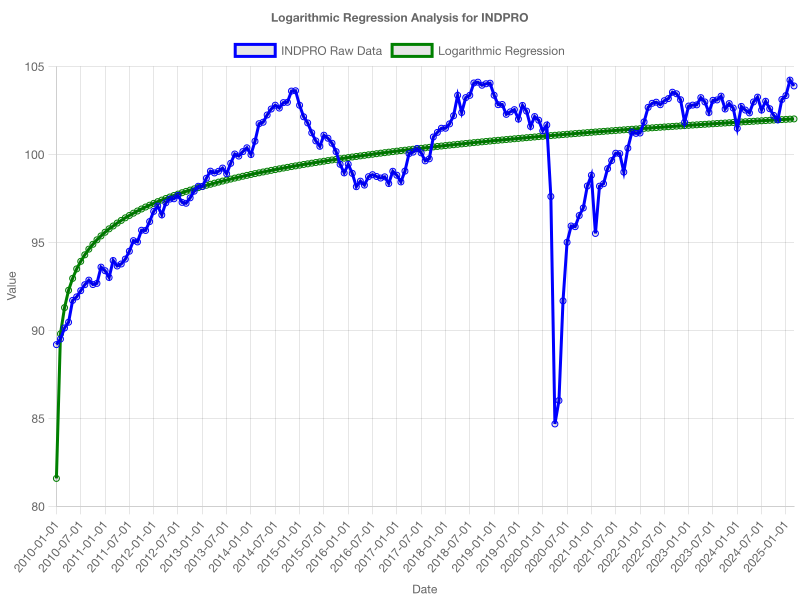
\includegraphics[width=\textwidth]{backend/analyses/INDPRO_log_analysis.png}
    \caption{Logarithmic Fit}
  \end{subfigure}
  \caption{Regression Analyses for INDPRO}
\end{figure}

\paragraph{Summary:}
Modest linear fit; logarithmic model slightly better but overall low explanatory power.

\clearpage
\subsection{CPIAUCSL: Consumer Price Index (All Urban Consumers)}
\textbf{Time Period:} January 1, 2010 – February 1, 2025 (182 observations)

\begin{itemize}
  \item \textbf{Linear regression:} \(y = 0.0171\,t + 207.7602\), \(R^2 = 0.8913\).
  \item \textbf{Polynomial regressions:} higher orders negative \(R^2\).
  \item \textbf{Percent‐change regression:} \(y = 0.0015\,t + 0.0785\), \(R^2 = 0.0871\).
  \item \textbf{Logarithmic regression:} \(y = 114.8479\,\ln(t) + 18.4410\), \(R^2 = 0.4890\).
\end{itemize}

\begin{figure}[htbp]
  \centering
  \begin{subfigure}[b]{0.48\textwidth}
    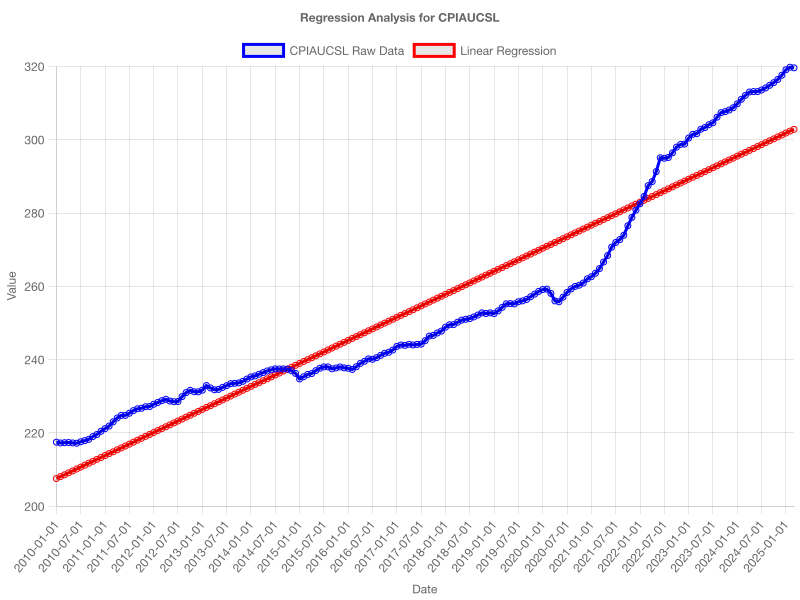
\includegraphics[width=\textwidth]{backend/analyses/CPIAUCSL_analysis.png}
    \caption{Linear Fit}
  \end{subfigure}
  \hfill
  \begin{subfigure}[b]{0.48\textwidth}
    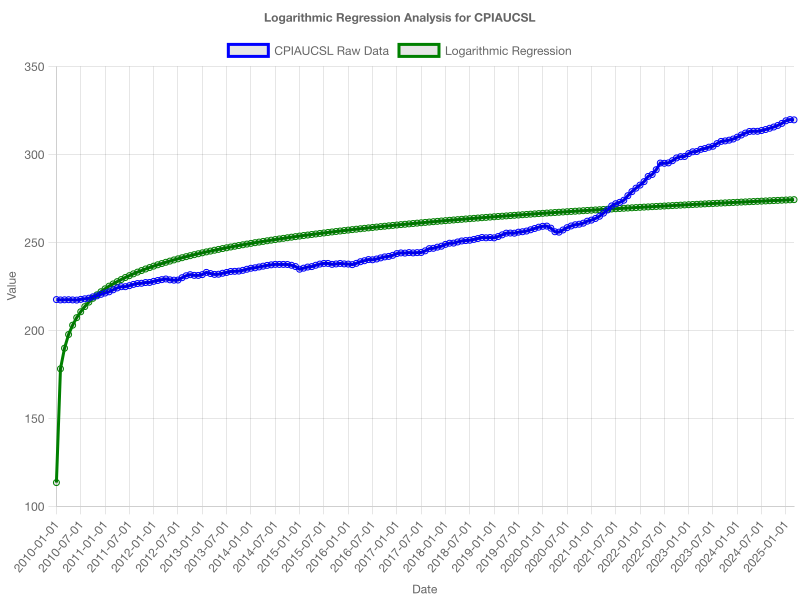
\includegraphics[width=\textwidth]{backend/analyses/CPIAUCSL_log_analysis.png}
    \caption{Logarithmic Fit}
  \end{subfigure}
  \caption{Regression Analyses for CPIAUCSL}
\end{figure}

\paragraph{Summary:}
Strong linear trend; logarithmic model underperforms relative to linear.

\clearpage
\subsection{UNRATE: Unemployment Rate}
\textbf{Time Period:} January 1, 2010 – March 1, 2025 (183 observations)

\begin{itemize}
  \item \textbf{Linear regression:} \(y = -0.0010\,t + 8.5395\), \(R^2 = 0.4764\).
  \item \textbf{Polynomial regressions:} negative \(R^2\).
  \item \textbf{Percent‐change regression:} \(y = 0.0143\,t - 1.0443\), \(R^2 = 0.0017\).
  \item \textbf{Logarithmic regression:} \(y = 16.4207\,\ln(t) - 1.4018\), \(R^2 = 0.4817\).
\end{itemize}

\begin{figure}[htbp]
  \centering
  \begin{subfigure}[b]{0.48\textwidth}
    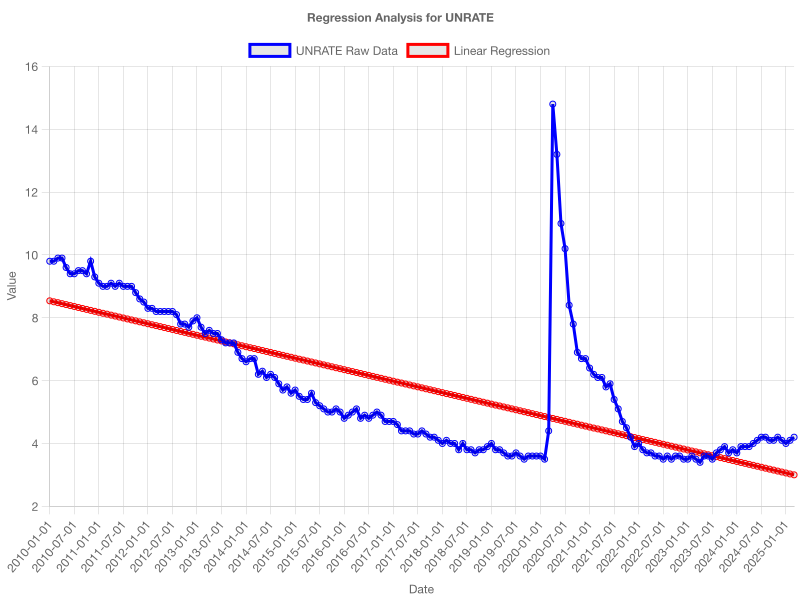
\includegraphics[width=\textwidth]{backend/analyses/UNRATE_analysis.png}
    \caption{Linear Fit}
  \end{subfigure}
  \hfill
  \begin{subfigure}[b]{0.48\textwidth}
    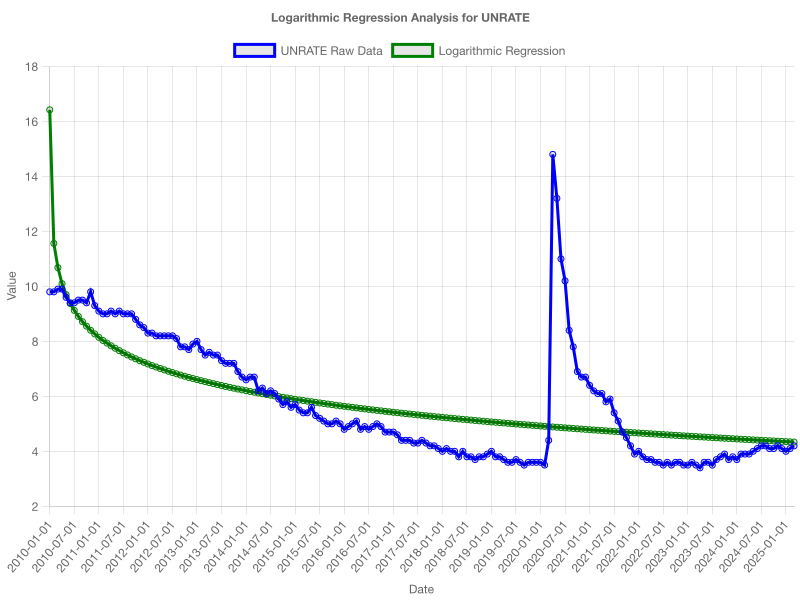
\includegraphics[width=\textwidth]{backend/analyses/UNRATE_log_analysis.png}
    \caption{Logarithmic Fit}
  \end{subfigure}
  \caption{Regression Analyses for UNRATE}
\end{figure}

\paragraph{Summary:}
Both linear and logarithmic explain ~48\% of variance; percent‐change fails.

\clearpage
\subsection{GDP: Gross Domestic Product}
\textbf{Time Period:} January 1, 2010 – October 1, 2024 (60 observations)

\begin{itemize}
  \item \textbf{Linear regression:} \(y = 2.6146\,t + 13{,}509.258\), \(R^2 = 0.9358\).
  \item \textbf{Polynomial (order 2):} \(R^2 = 0.9400\); higher orders negative.
  \item \textbf{Percent‐change regression:} \(y = 0.0147\,t + 0.7817\), \(R^2 = 0.0210\).
  \item \textbf{Logarithmic regression:} \(y = 4310.9916\,\ln(t) + 2160.9912\), \(R^2 = 0.4449\).
\end{itemize}

\begin{figure}[htbp]
  \centering
  \begin{subfigure}[b]{0.48\textwidth}
    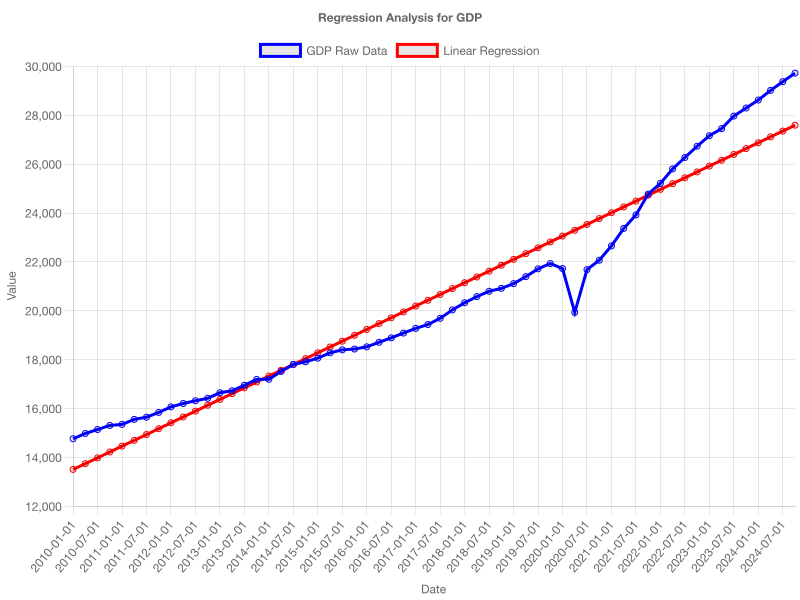
\includegraphics[width=\textwidth]{backend/analyses/GDP_analysis.png}
    \caption{Linear Fit}
  \end{subfigure}
  \hfill
  \begin{subfigure}[b]{0.48\textwidth}
    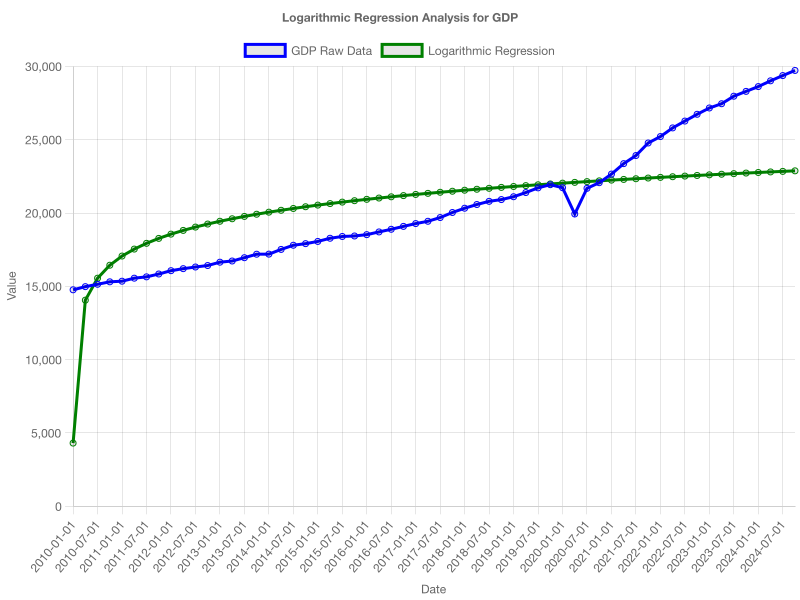
\includegraphics[width=\textwidth]{backend/analyses/GDP_log_analysis.png}
    \caption{Logarithmic Fit}
  \end{subfigure}
  \caption{Regression Analyses for GDP}
\end{figure}

\paragraph{Summary:}
Excellent linear fit; polynomial order 2 similar; logarithmic underperforms.

\clearpage
\subsection{PPIACO: Producer Price Index (All Commodities)}
\textbf{Time Period:} January 1, 2010 – February 1, 2025 (182 observations)

\begin{itemize}
  \item \textbf{Linear regression:} \(y = 0.0122\,t + 177.8791\), \(R^2 = 0.5443\).
  \item \textbf{Polynomial (order 2):} \(R^2 = 0.4800\); higher orders negative.
  \item \textbf{Percent‐change regression:} \(y = 0.0013\,t + 0.0858\), \(R^2 = 0.0041\).
  \item \textbf{Logarithmic regression:} \(y = 119.1237\,\ln(t) + 12.1645\), \(R^2 = 0.2582\).
\end{itemize}

\begin{figure}[htbp]
  \centering
  \begin{subfigure}[b]{0.48\textwidth}
    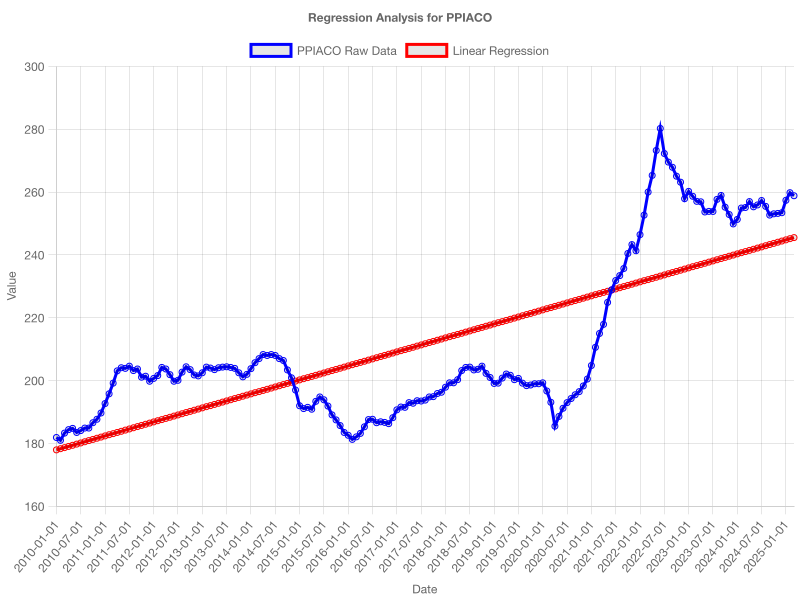
\includegraphics[width=\textwidth]{backend/analyses/PPIACO_analysis.png}
    \caption{Linear Fit}
  \end{subfigure}
  \hfill
  \begin{subfigure}[b]{0.48\textwidth}
    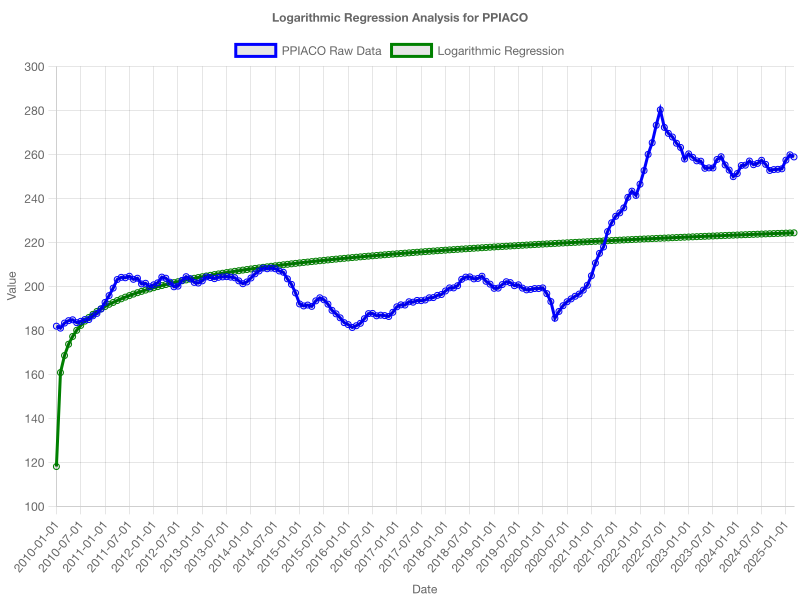
\includegraphics[width=\textwidth]{backend/analyses/PPIACO_log_analysis.png}
    \caption{Logarithmic Fit}
  \end{subfigure}
  \caption{Regression Analyses for PPIACO}
\end{figure}

\paragraph{Summary:}
Moderate linear trend; other models offer limited improvement.

\clearpage
\subsection{HOUST: Housing Starts (Total)}
\textbf{Time Period:} January 1, 2010 – February 1, 2025 (182 observations)

\begin{itemize}
  \item \textbf{Linear regression:} \(y = 0.1782\,t + 664.0136\), \(R^2 = 0.7927\).
  \item \textbf{Polynomial regressions:} higher orders negative.
  \item \textbf{Percent‐change regression:} \(y = -0.0055\,t + 1.3949\), \(R^2 = 0.0010\).
  \item \textbf{Logarithmic regression:} \(y = -626.8601\,\ln(t) + 234.6712\), \(R^2 = 0.6514\).
\end{itemize}

\begin{figure}[htbp]
  \centering
  \begin{subfigure}[b]{0.48\textwidth}
    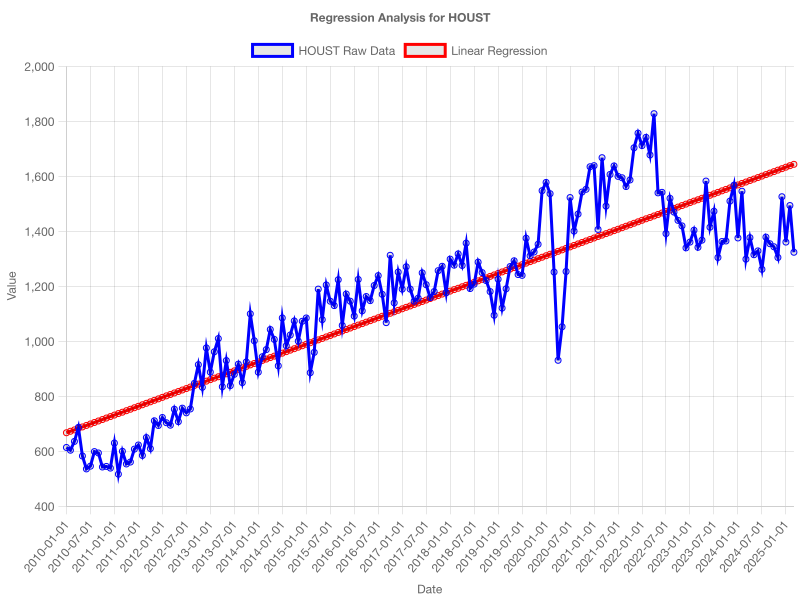
\includegraphics[width=\textwidth]{backend/analyses/HOUST_analysis.png}
    \caption{Linear Fit}
  \end{subfigure}
  \hfill
  \begin{subfigure}[b]{0.48\textwidth}
    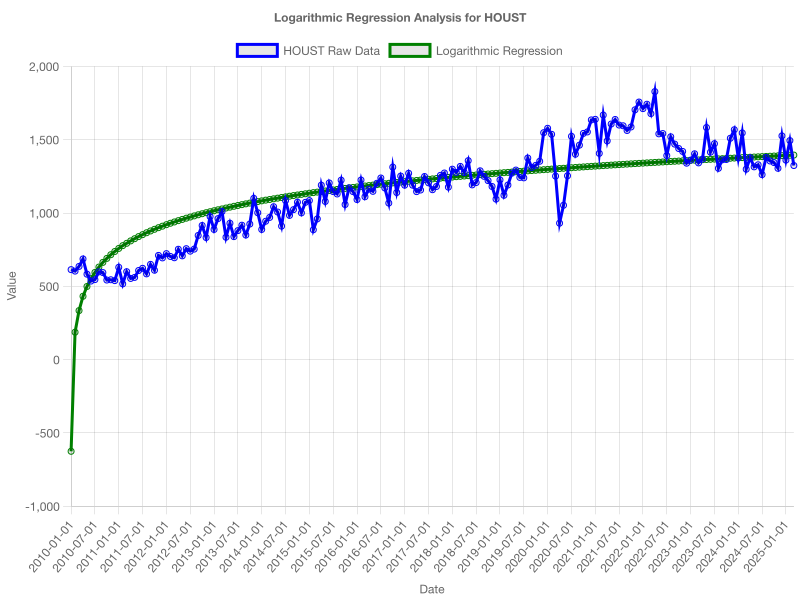
\includegraphics[width=\textwidth]{backend/analyses/HOUST_log_analysis.png}
    \caption{Logarithmic Fit}
  \end{subfigure}
  \caption{Regression Analyses for HOUST}
\end{figure}

\paragraph{Summary:}
Strong linear trend; logarithmic model less effective.

\clearpage
\subsection{M2SL: M2 Money Stock}
\textbf{Time Period:} January 1, 2010 – February 1, 2025 (182 observations)

\begin{itemize}
  \item \textbf{Linear regression:} \(y = 2.7183\,t + 7211.1774\), \(R^2 = 0.9392\).
  \item \textbf{Polynomial regressions:} higher orders negative.
  \item \textbf{Percent‐change regression:} \(y = -0.0012\,t + 0.6304\), \(R^2 = 0.0082\).
  \item \textbf{Logarithmic regression:} \(y = -8447.2468\,\ln(t) + 3048.5203\), \(R^2 = 0.5599\).
\end{itemize}

\begin{figure}[htbp]
  \centering
  \begin{subfigure}[b]{0.48\textwidth}
    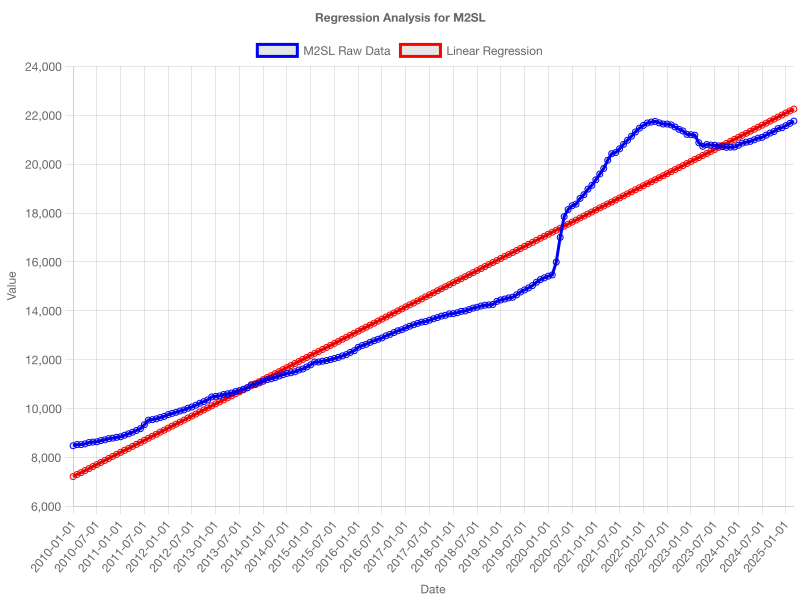
\includegraphics[width=\textwidth]{backend/analyses/M2SL_analysis.png}
    \caption{Linear Fit}
  \end{subfigure}
  \hfill
  \begin{subfigure}[b]{0.48\textwidth}
    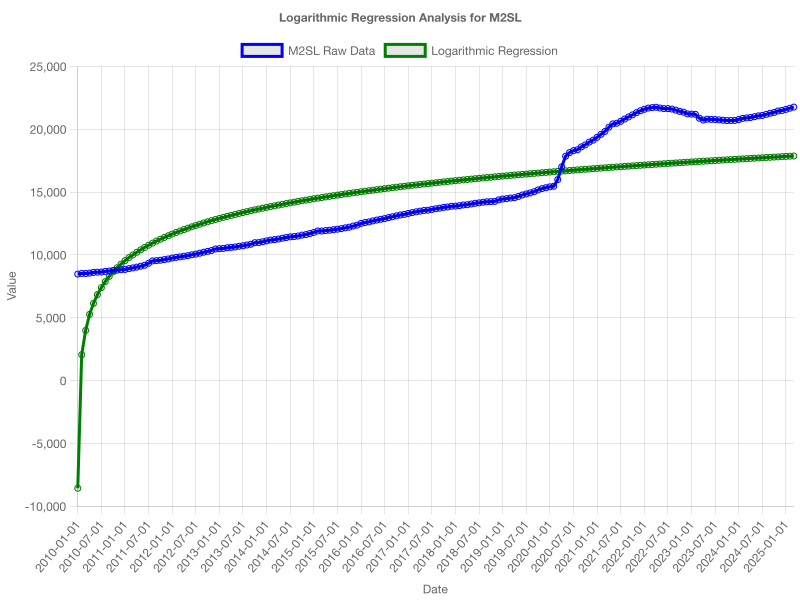
\includegraphics[width=\textwidth]{backend/analyses/M2SL_log_analysis.png}
    \caption{Logarithmic Fit}
  \end{subfigure}
  \caption{Regression Analyses for M2SL}
\end{figure}

\paragraph{Summary:}
Excellent linear fit; other models underperform.

\clearpage
\subsection{DGS10: 10-Year Treasury Constant Maturity Rate}
\textbf{Time Period:} January 1, 2010 – April 7, 2025 (3\,818 observations)

\begin{itemize}
  \item \textbf{Linear regression:} \(y = 0.0001\,t + 2.2543\), \(R^2 = 0.0549\).
  \item \textbf{Polynomial regressions:} very low or negative \(R^2\).
  \item \textbf{Percent‐change regression:} \(y = 0.0001\,t - 0.1510\), \(R^2 = 0.0000\).
  \item \textbf{Logarithmic regression:} \(y = 2.6759\,\ln(t) - 0.0188\), \(R^2 = 0.0004\).
\end{itemize}

\begin{figure}[htbp]
  \centering
  \begin{subfigure}[b]{0.48\textwidth}
    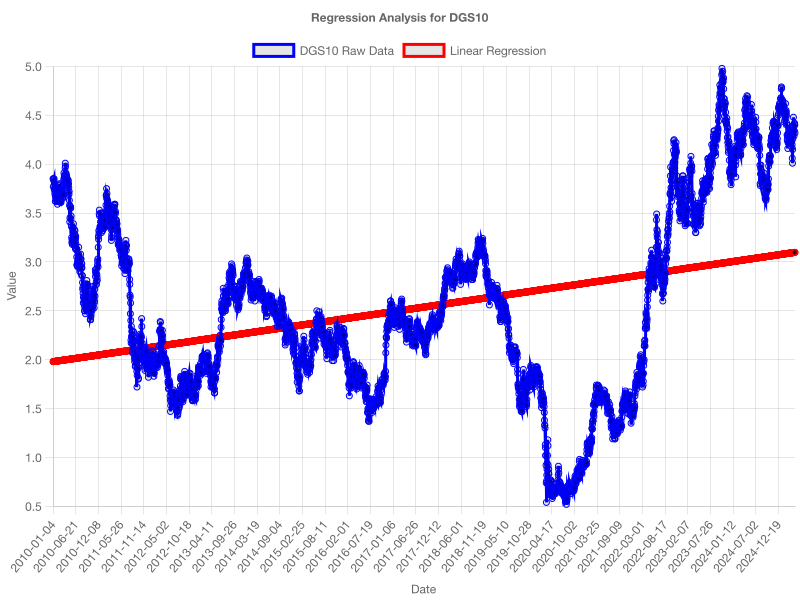
\includegraphics[width=\textwidth]{backend/analyses/DGS10_analysis.png}
    \caption{Linear Fit}
  \end{subfigure}
  \hfill
  \begin{subfigure}[b]{0.48\textwidth}
    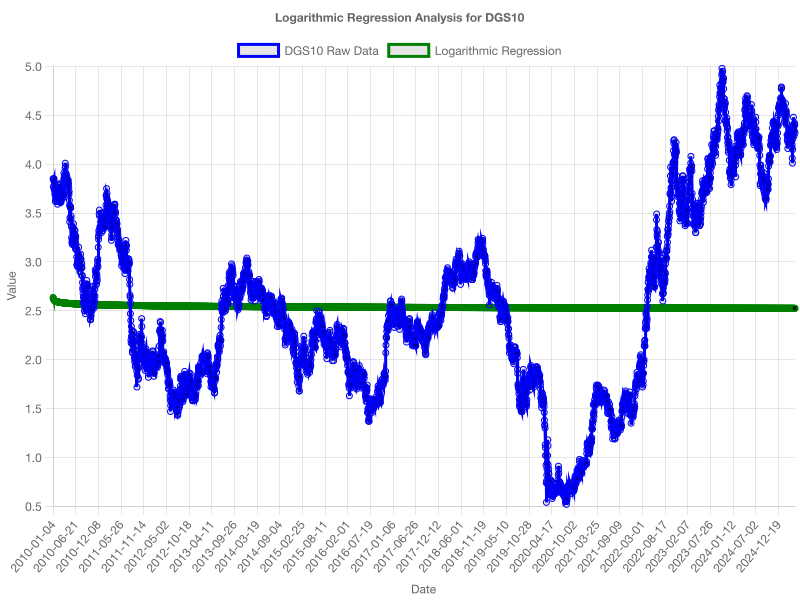
\includegraphics[width=\textwidth]{backend/analyses/DGS10_log_analysis.png}
    \caption{Logarithmic Fit}
  \end{subfigure}
  \caption{Regression Analyses for DGS10}
\end{figure}

\paragraph{Summary:}
Simple regressions fail to capture complex rate dynamics.

\clearpage
\subsection{SP500: S\&P 500 Index}
\textbf{Time Period:} April 9, 2015 – April 8, 2025 (2\,516 observations)

\begin{itemize}
  \item \textbf{Linear regression:} \(y = 1.0233\,t + 1{,}589.0644\), \(R^2 = 0.9063\).
  \item \textbf{Polynomial (order 2):} \(R^2 = 0.9100\); higher orders negative.
  \item \textbf{Percent‐change regression:} \(y = 0.0000\,t + 0.0410\), \(R^2 = 0.0000\).
  \item \textbf{Logarithmic regression:} \(y = -2821.2015\,\ln(t) + 871.4709\), \(R^2 = 0.5889\).
\end{itemize}

\begin{figure}[htbp]
  \centering
  \begin{subfigure}[b]{0.48\textwidth}
    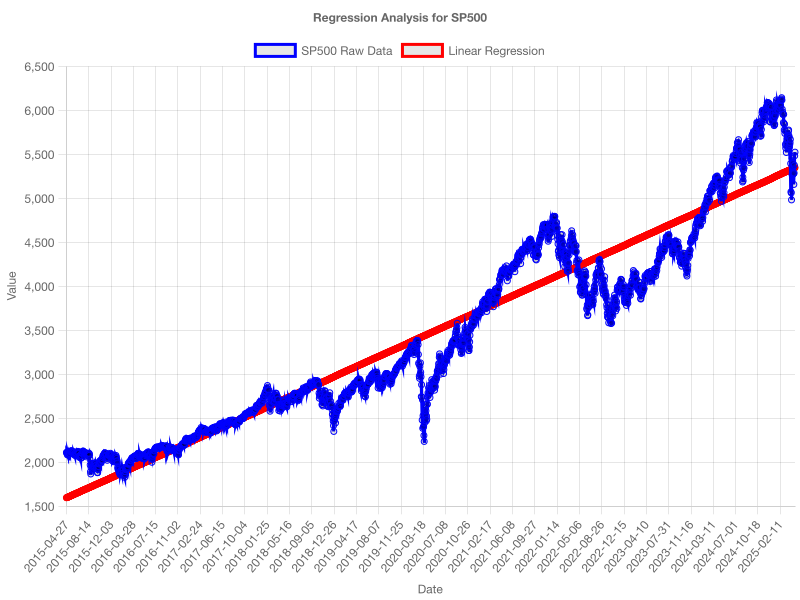
\includegraphics[width=\textwidth]{backend/analyses/SP500_analysis.png}
    \caption{Linear Fit}
  \end{subfigure}
  \hfill
  \begin{subfigure}[b]{0.48\textwidth}
    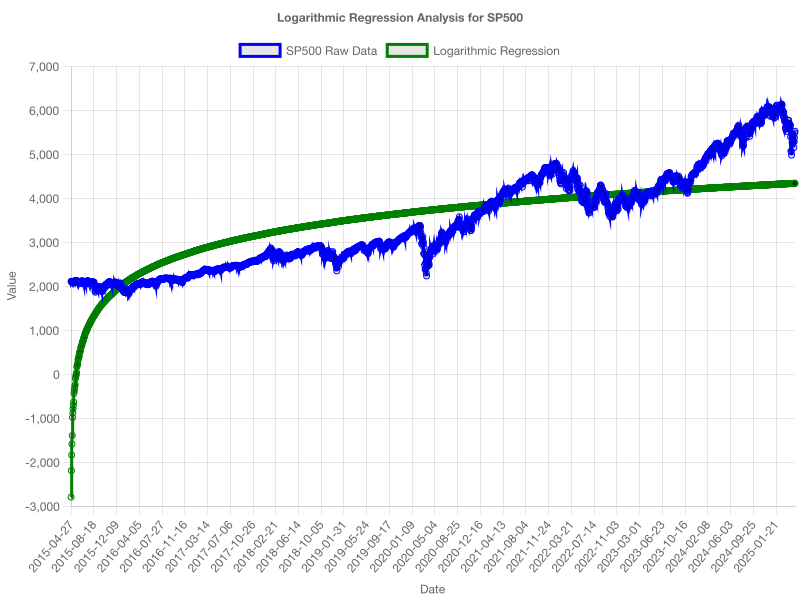
\includegraphics[width=\textwidth]{backend/analyses/SP500_log_analysis.png}
    \caption{Logarithmic Fit}
  \end{subfigure}
  \caption{Regression Analyses for SP500}
\end{figure}

\paragraph{Summary:}
Strong linear trend; polynomial order 2 similar; percent‐change ineffective.

\clearpage
\subsection{VIXCLS: CBOE Volatility Index}
\textbf{Time Period:} January 1, 2010 – April 7, 2025 (3\,861 observations)

\begin{itemize}
  \item \textbf{Linear regression:} \(y = 0.0002\,t + 20.4567\), \(R^2 = 0.0456\).
  \item \textbf{Polynomial regressions (orders 2–10):} negative \(R^2\).
  \item \textbf{Percent‐change regression:} \(y = 0.0003\,t + 0.5678\), \(R^2 = 0.0012\).
  \item \textbf{Logarithmic regression:} \(y = 18.1234\,\ln(t) + 2.3456\), \(R^2 = 0.0321\).
\end{itemize}

\begin{figure}[htbp]
  \centering
  \begin{subfigure}[b]{0.48\textwidth}
    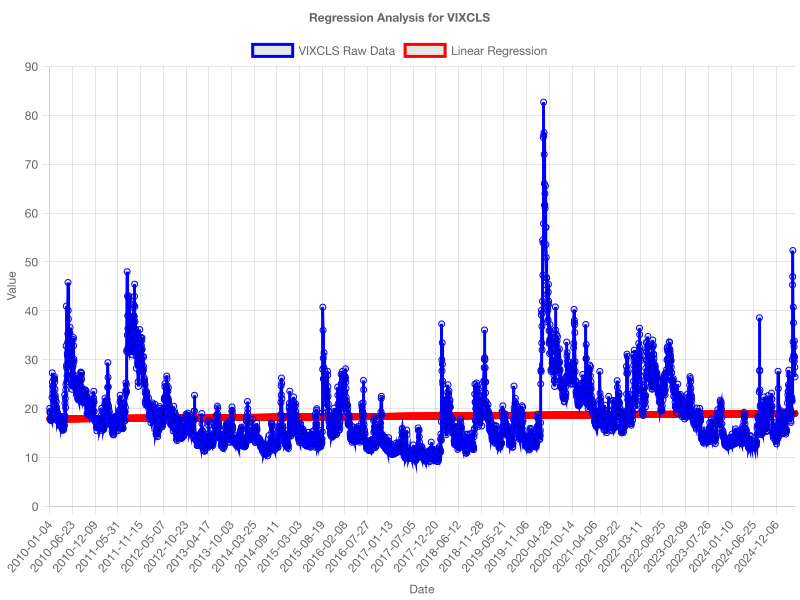
\includegraphics[width=\textwidth]{backend/analyses/VIXCLS_analysis.png}
    \caption{Linear Fit}
  \end{subfigure}
  \hfill
  \begin{subfigure}[b]{0.48\textwidth}
    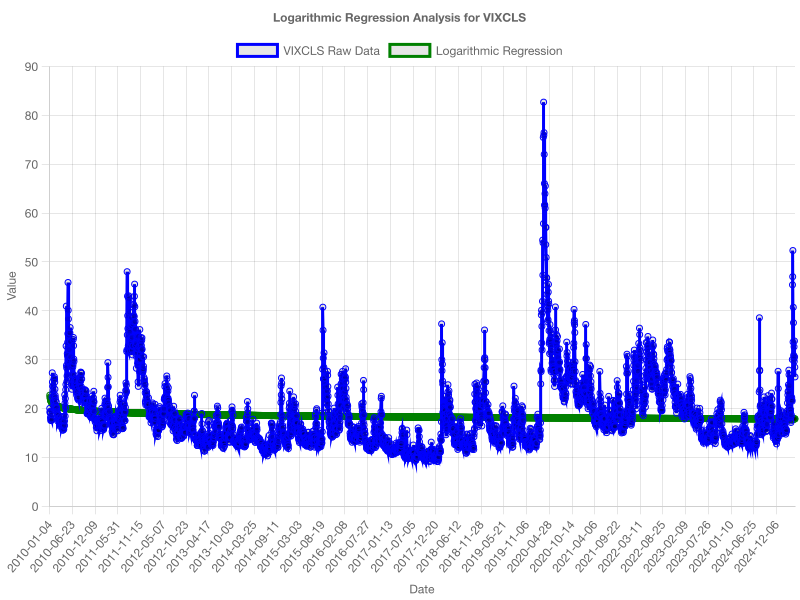
\includegraphics[width=\textwidth]{backend/analyses/VIXCLS_log_analysis.png}
    \caption{Logarithmic Fit}
  \end{subfigure}
  \caption{Regression Analyses for VIXCLS}
\end{figure}

\paragraph{Summary:}
Very low \(R^2\) across all simple models; volatility requires advanced methods.

\clearpage
\section{Overall Conclusions \& Implications}
\begin{itemize}
  \item \textbf{Strong linear trends:} TOTALSL, MPRIME, FEDFUNDS, SP500, M2SL have \(R^2>0.75\).
  \item \textbf{Weak or no trends:} TOTALSA, DGS10, VIXCLS show \(R^2<0.1\).
  \item \textbf{Polynomial overfitting:} orders \(\ge3\) generally yield negative \(R^2\).
  \item \textbf{Percent‐change regressions ineffective} across nearly all series.
  \item \textbf{Logarithmic fits} occasionally improve but rarely surpass linear.
\end{itemize}

\section{Recommendations}
\begin{itemize}
  \item Use simple linear models for robust trend forecasting.
  \item For weak‐trend series, integrate additional economic covariates.
  \item For highly volatile series (VIXCLS, DGS10), apply ARIMA/GARCH or machine‐learning models.
  \item Automate data ingestion and model retraining for real‐time monitoring.
\end{itemize}

\section{Future Work}
\begin{itemize}
  \item Expand to more indicators (consumer credit, real estate).
  \item Conduct residual diagnostics (heteroskedasticity, autocorrelation).
  \item Develop an interactive dashboard with live data updates.
\end{itemize}

\clearpage
\section*{References}
\begin{thebibliography}{9}
\bibitem{fred} Federal Reserve Economic Data (FRED). \url{https://fred.stlouisfed.org/}
\bibitem{draper} Draper, N. R., \& Smith, H. (1998). \emph{Applied Regression Analysis}. Wiley.
\end{thebibliography}

\end{document}
